\documentclass[a4paper]{report}
\usepackage[margin=3.5cm]{geometry}
\usepackage[svgnames]{xcolor}
\usepackage{amsmath,amsfonts,amssymb,amsthm,thmtools,thm-restate}
\usepackage{graphicx,dsfont,hyperref,datetime,float,booktabs,enumitem,outlines}
\usepackage{nicemat
  rix}
\usepackage[activate={true,nocompatibility},final,tracking=true,kerning=true,spacing=true,factor=500,stretch=15,shrink=15]{microtype}

\usepackage{titlesec}

% \titleformat{\chapter}  % which section command to format
%   {\fontsize{18}{20}\bfseries} % format for whole line
%   {Chapter \thechapter} % how to show number
%   {1em} % space between number and text
%   {} % formatting for just the text
%   [] % formatting for after the text

\titleformat{\chapter}[display]
{\normalfont\fontsize{18}{20}\bfseries}
{\chaptertitlename\ \thechapter }
{15pt}{\huge} % changed
\titlespacing*{\chapter}{0pt}{-15pt}{20pt}  % changed

\titleformat{\section}  % which section command to format
  {\fontsize{14}{15}\bfseries} % format for whole line
  {\thesection} % how to show number
  {1em} % space between number and text
  {} % formatting for just the text
  [] % formatting for after the text

\titleformat{\subsection}  % which section command to format
  {\fontsize{12}{14}\bfseries} % format for whole line
  {\thesubsection} % how to show number
  {1em} % space between number and text
  {} % formatting for just the text
  [] % formatting for after the text

% load knitr
\definecolor{fgcolor}{rgb}{0.345, 0.345, 0.345}
\newcommand{\hlnum}[1]{\textcolor[rgb]{0.686,0.059,0.569}{#1}}%
\newcommand{\hlstr}[1]{\textcolor[rgb]{0.192,0.494,0.8}{#1}}%
\newcommand{\hlcom}[1]{\textcolor[rgb]{0.678,0.584,0.686}{\textit{#1}}}%
\newcommand{\hlopt}[1]{\textcolor[rgb]{0,0,0}{#1}}%
\newcommand{\hlstd}[1]{\textcolor[rgb]{0.345,0.345,0.345}{#1}}%
\newcommand{\hlkwa}[1]{\textcolor[rgb]{0.161,0.373,0.58}{\textbf{#1}}}%
\newcommand{\hlkwb}[1]{\textcolor[rgb]{0.69,0.353,0.396}{#1}}%
\newcommand{\hlkwc}[1]{\textcolor[rgb]{0.333,0.667,0.333}{#1}}%
\newcommand{\hlkwd}[1]{\textcolor[rgb]{0.737,0.353,0.396}{\textbf{#1}}}%
\let\hlipl\hlkwb

\usepackage{framed}
\makeatletter
\newenvironment{kframe}{%
 \def\at@end@of@kframe{}%
 \ifinner\ifhmode%
  \def\at@end@of@kframe{\end{minipage}}%
  \begin{minipage}{\columnwidth}%
 \fi\fi%
 \def\FrameCommand##1{\hskip\@totalleftmargin \hskip-\fboxsep
 \colorbox{shadecolor}{##1}\hskip-\fboxsep
     % There is no \\@totalrightmargin, so:
     \hskip-\linewidth \hskip-\@totalleftmargin \hskip\columnwidth}%
 \MakeFramed {\advance\hsize-\width
   \@totalleftmargin\z@ \linewidth\hsize
   \@setminipage}}%
 {\par\unskip\endMakeFramed%
 \at@end@of@kframe}
\makeatother

\definecolor{shadecolor}{rgb}{.97, .97, .97}
\definecolor{messagecolor}{rgb}{0, 0, 0}
\definecolor{warningcolor}{rgb}{1, 0, 1}
\definecolor{errorcolor}{rgb}{1, 0, 0}
\newenvironment{knitrout}{}{} % an empty environment to be redefined in TeX


% theorem environments
\theoremstyle{definition}
\newtheorem{eg}{Example}
\newtheorem{define}{Definition}[section]
\theoremstyle{plain}
\newtheorem{proposition}{Proposition}[section]
\newtheorem{lemma}{Lemma}[section]
\newtheorem{theorem}{Theorem}[section]
\newtheorem{assump}{Assumption}[section]
\newtheorem{remark}{Remark}[section]

\newdateformat{monthyeardate}{\monthname[\THEMONTH] \THEYEAR}
\author{Jeroen van Riel}
\date{\monthyeardate\today}
\title{%
  \huge Machine Learning Scheduling for the Coordination of Automated Vehicles
  }

\newcommand\halfopen[2]{\ensuremath{[#1,#2)}}
\newcommand\openhalf[2]{\ensuremath{(#1,#2]}}

\begin{document}

% \begin{minipage}[h]{\textwidth}
%     \maketitle
%     \begin{center}
%     \textbf{Abstract}
%     \end{center}
%     Coordination of automated vehicles in a network of intersections is modeled
%     as a trajectory optimization problem. Under certain model assumptions, this
%     problem can be decomposed into (i) an upper-level scheduling problem of
%     determining the crossing times at intersections and (ii) a set of
%     lower-level trajectory optimization problems. We show that the feasibility
%     of the lower-level problems is characterized as a set of linear inequalities
%     in the crossing times.
%     %
%     Since schedules can be interpreted as a sequence of discrete decisison, we
%     experiment with sequence modeling to solve the crossing time scheduling. We
%     compare a simple parameterization with a neural network model. As previously
%     observed by others, our case study illustrates that the evaluation order of
%     the sequence model matters for the final performance.
% \end{minipage}

% \begin{figure}[b!]
%   \centering
%   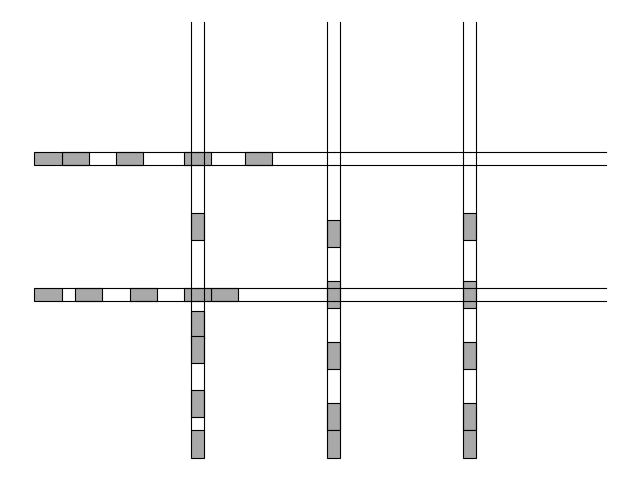
\includegraphics[width=0.7\textwidth]{figures/network/grid_example.png}
% \end{figure}

% \tableofcontents

% \chapter*{Preface}
% \addcontentsline{toc}{chapter}{\protect\numberline{}Preface}

% Special thanks to Erjen Lefeber for his involvement in the analysis of the single lane model.

% All hand-drawn figures in this thesis were produced by the Ipe extensible
% drawing editor\footnote{\url{https://ipe.otfried.org}}.


\chapter{Introduction and background}

\section{Introduction}

% motivation
% automated vehicles

Given the ongoing advances in self-driving vehicles and wireless communication,
it is very natural to study how these new technologies can be applied to enable
network-wide traffic coordination.
%
Some of the potential benefits of coordinating the motion of groups of automated
vehicles are increased network throughput, reduced energy consumption and better
guarantees on safety in terms of avoiding dangerous situations.

Coordination of automated vehicles with communication has been studied at
various levels of organization~\cite{marianiCoordinationAutonomousVehicles2022}.
A good example of a local coordination methods is platooning of vehicles, where
the aim is to lower energy consumption by reducing aerodynamic resistance. It
has been shown that platooning can also result in a more efficient use of
intersections. On a larger scale, methods like dynamic route optimization have
been proposed to reduce travel delay for all vehicles in the network.
%
The coordination problem has very many aspects that could be modeled and
analyzed. For example, one may think of heterogenous vehicles---in terms of
dynamics or priority---different models of centralized/decentralized
communication between vehicles or with the infrastructure, under different
guarantees on reliability; complex road topology, curved lanes, merging lanes.

However, as we will see, even the most basic models already present fundamental
challenges in ensuring safety and efficiency.
%
Therefore, we will only consider the two most essential elements in this thesis,
being vehicle dynamics and the constraints that are required to model the
allowed paths vehicles may take in order to avoid collisions with the
infrastructure and other vehicles.
%
To keep things simple, we assume that all vehicles are automated and share the
same dynamics.
%
Each vehicle follows a fixed route through the network and is centrally
controlled through acceleration inputs under the assumption of perfect
communication.
%
With these assumptions, the traffic coordination task can be modeled a
trajectory optimization problem.
%
To illustrate the kind of model that we will study, we present a concrete
minimal example of a single intersection with two vehicles.

\begin{figure}
  \centering
  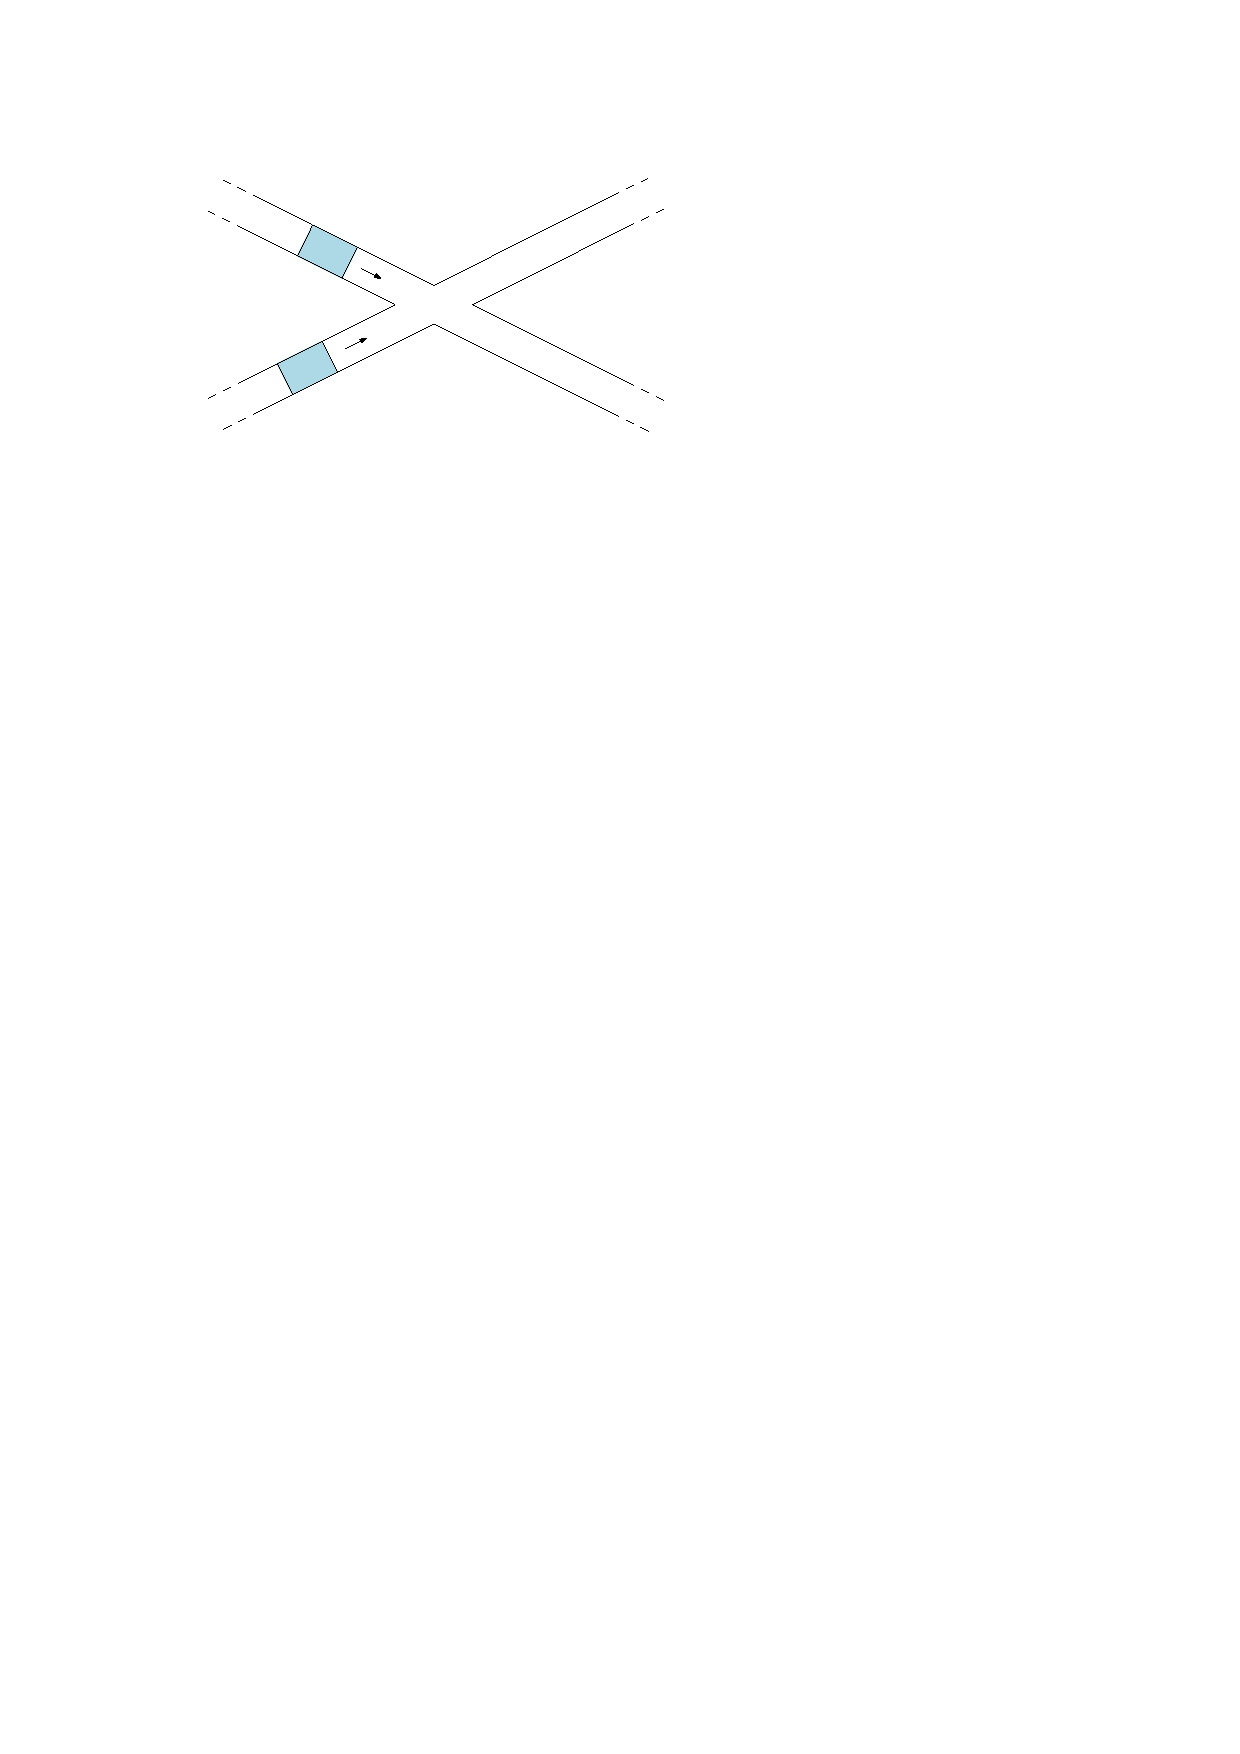
\includegraphics[scale=1]{figures/intersection-non-axis-aligned}
  \caption{Example of two lanes intersection intersecting at some angle
    $\alpha$. The indicated positions $B_{i}$ and $E_{i}$ for each vehicle $i$
    are such that if the front bumper position $x_{i}$ satisfies either
    $x_{i} \leq B_{i}$ or $x_{i} - L \geq E_{i}$, then the intersection area is
    guaranteed to be completely free.}%
  \label{fig:intersection-non-axis-aligned}
\end{figure}

% concrete illustration
\paragraph{Intersection model.}

Consider two vehicles, modeled as rigid bodies of width $W$ and length $L$, each
driving on its own straight lane of width $W$ and infinite length.
%
Suppose that the lanes intersect at some angle $\alpha$, as shown in
Figure~\ref{fig:intersection-non-axis-aligned}.
%
To uniquely define the position of each vehicle $i \in \{1, 2\}$ on its lane, we
use $x_{i} \in \mathbb{R}$ to denote the position of its front bumper. Hence,
$x_{i} - L$ is the position of the rear bumper.

We might try to characterize the set $\mathcal{X} \subset \mathbb{R}^{2}$ of all
feasible configurations $(x_{1}, x_{2})$ for which the two vehicles do not
intersect.
%
% discuss rectangular subset of configuration space
%
Fix the positions $x_{i} = B_{i}$ and $x_{i} = E_{i}$, as shown in
Figure~\ref{fig:intersection-non-axis-aligned}.
%
Whenever we have $x_{i} \leq B_{i}$ or $x_{i} - L \geq E_{i}$, it is clear that
vehicle $i$ does not occupy the intersection at all, so the other vehicle $j$ is
free to take any position $x_{j} \in \mathbb{R}$. Therefore, whenever
$x_{1} \notin (B_{1},E_{1})$ and $x_{2} \notin (B_{2}, E_{2})$, we know for sure
that $(x_{1}, x_{2})$ is a feasible configuration. Hence, we readily obtain some
subset of feasible configurations
\begin{align}\label{eq:conf-space-subset}
  \mathbb{R}^{2} \setminus ((B_{1},E_{1}) \times (B_{2},E_{2})) \subset \mathcal{X} .
\end{align}
In general, the set of feasible configurations is a little larger, as
illustrated by the three examples in
Figure~\ref{fig:intersection-config-spaces}.
%
In case of the third example, when the intersections make a right angle, it can
be shown that there is equality in~\eqref{eq:conf-space-subset}, which makes
subsequent analysis easier.

We now discuss the dynamics of the vehicles, so let $x_{i}(t)$ denote the
position of vehicle $i$ at time $t$.
%
Let $\dot{x}_{i}$ and $\ddot{x}_{i}$ denote the speed and acceleration of
vehicle $i$, respectively, and consider the following bounds
\begin{align}\label{eq:vehicle-dynamics}
  \dot{x}_{i}(t) \in [\hspace{0.05em} 0, 1] , \quad\quad  \ddot{x}_{i}(t) \in [\hspace{0.1em} -\bar{\omega}, \omega \, ] ,
\end{align}
for some positive $\bar{\omega}, \omega > 0$.
%
Assume the initial vehicle state
$(x_{i}(0), \dot{x}_{i}(0)) = (x_{i}^{0}, \dot{x}_{i}^{0})$ is fixed.

Let $J(x_{i})$ be some functional that measures how desirable trajectory
$x_{i}(t)$ is.
%
Given some final
simulation time $T > 0$, we consider the problem of maximizing
$J(x_{1}) + J(x_{2})$ such that $(x_{1}(t), x_{2}(t)) \in \mathcal{X}$ and the
bounds~\eqref{eq:vehicle-dynamics} hold for all times $t \in [0, T]$.
%
It is easy to see that this optimization problem is non-convex, because the
space of feasible configurations $\mathcal{X}$ is non-convex.
%
An interpretation of this non-convexity is that we must decide which of the
vehicles crosses the intersection first.

\begin{figure}
  \centering
  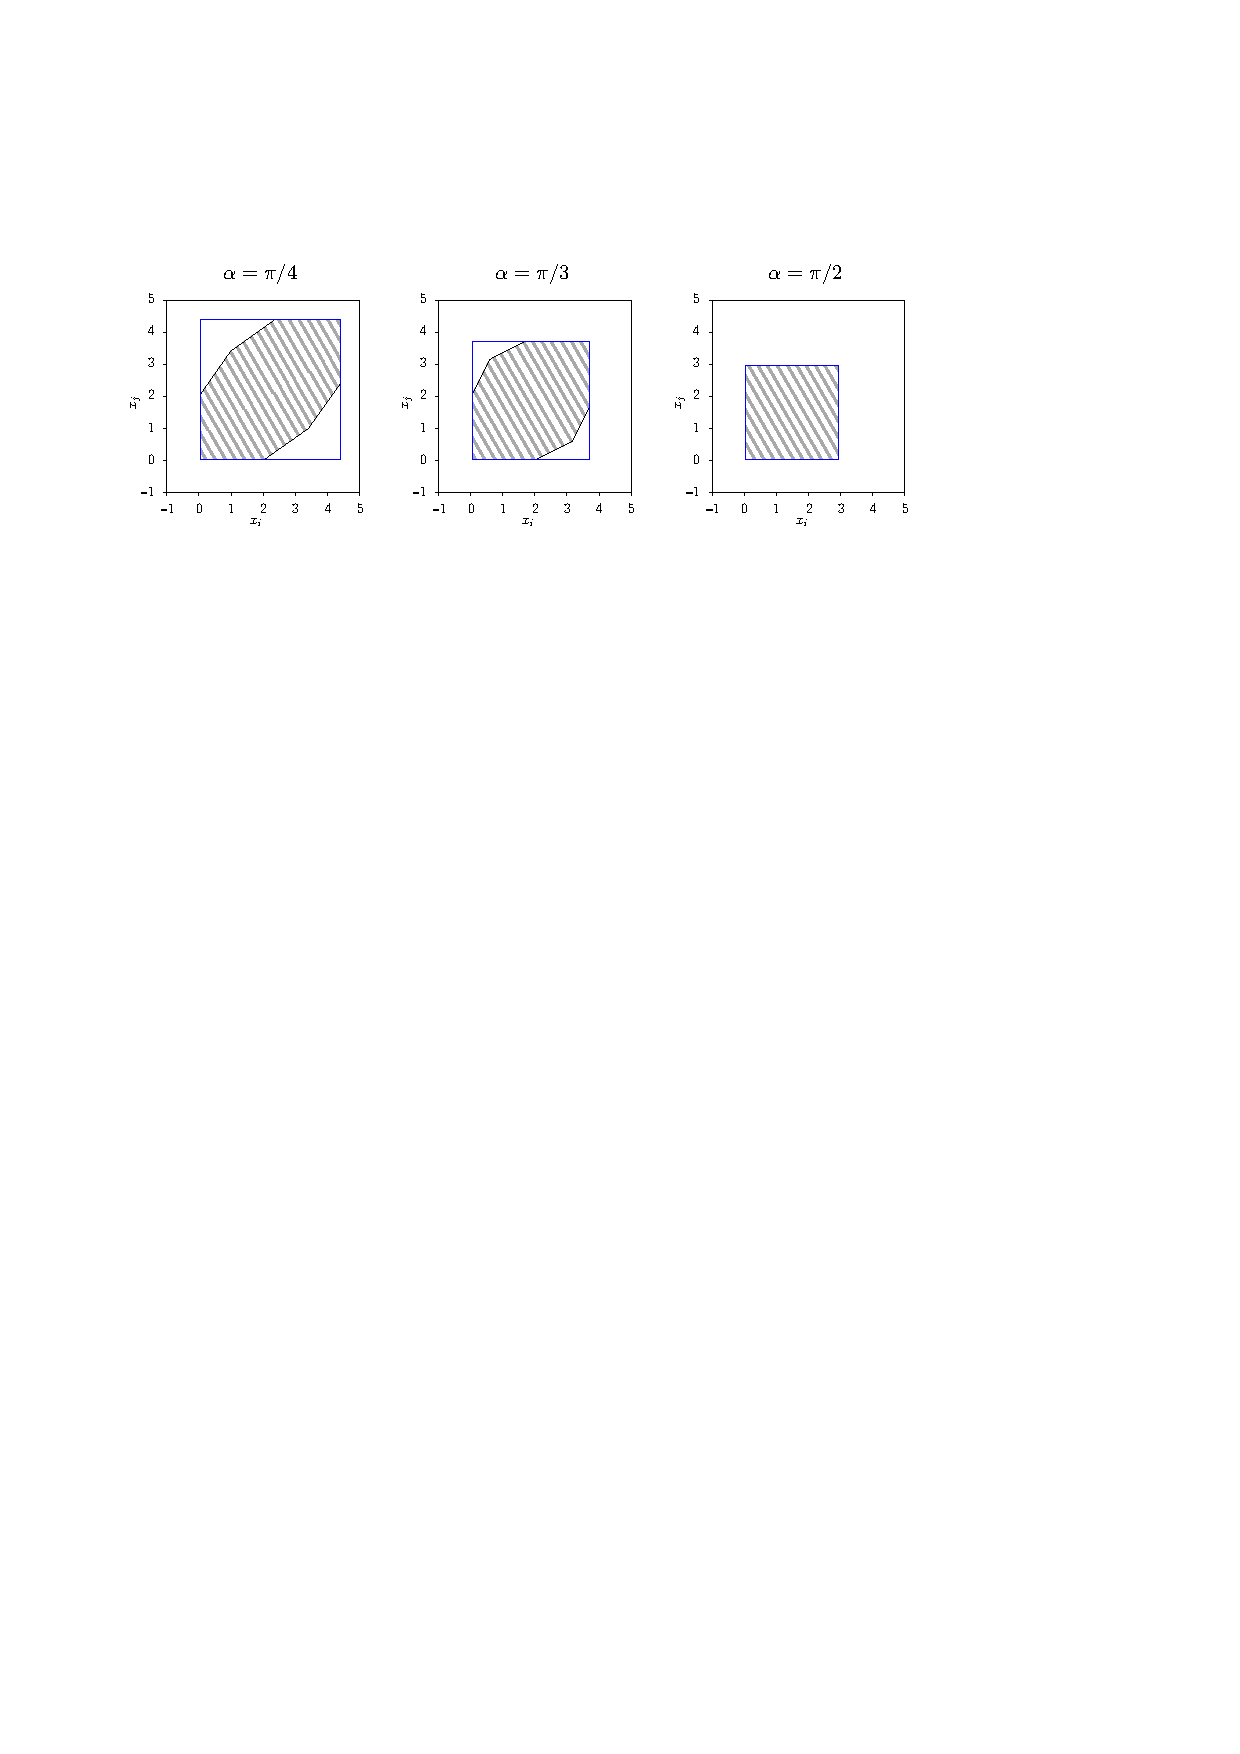
\includegraphics[scale=1]{figures/intersection-config-spaces}
  \caption{The first row shows three instances of the intersection model with
    for three different angles $\alpha_{k}$ and fixed vehicle dimenions $W=1$
    and $L=2$. Below each model, we plotted the region in configuration space
    space corresponding to collisions, marked in blue. We briefly explain our
    method to compute these plots in Appendix~\ref{app:configuration-space}.}%
  \label{fig:intersection-config-spaces}
\end{figure}


\paragraph{Crossing time scheduling.} As the example shows, we need to take a
discrete decision regarding the crossing order of vehicles at intersections.
This remains true for any generalization of the model to multiple lanes and
intersections.
%
However, after fixing these ordering decisions, the remaining problem is often
much easier to solve. This observation motivates the decomposition of the
trajectory optimization problem into two parts.
%
The upper-level problem determines the times at which vehicles cross the
intersections on their routes, to which we will refer as \emph{crossing times}.
%
Once these are fixed, we solve a set of lower-level problems to find the
corresponding vehicle trajectories satisfying the crossing times.

Without additional assumptions, the upper-level problem is still as difficult as
before, because the feasibility of a crossing time schedule may depend on the
feasibility of the lower-level trajectory optimization problems in a non-trivial
way.
%
We will provide assumptions under which this coupling becomes particularly
simple.
%
Specifically, we show that feasibility of the lower-level problems can be states
as a system of linear inequalities in terms of the crossing times and we will
see that they also have simple interpretations.
%
This allows us to formulate the upper-level problem as a mixed-integer linear
problem that looks very similar to the classical job shop scheduling problem.

\paragraph{Learning to schedule.}

Because the lower-level problems can in general be solved efficiently, the
original trajectory optimization problem is essentially reduced to a scheduling
problem.
%
This enables us to explore some applictions of recent machine learning
techniques for such problems.
%
Specifically, the solution of a scheduling problem can be interpreted as a
sequence of decisions.
%
Instead of manually trying to develop good heuristics and algorithms, we try to
learn what optimal solutions are, by treating it as a learning task on
sequences.


\subsection{Related work}

We briefly survey some releated work that addressed coordination of autonomous
vehicles in a similar setting.
%
A good example of an early centralized approach
is the ``Autonomous Intersection Management'' (AIM)
paper~\cite{dresnerMultiagentApproachAutonomous2008}, which is based on a
reservation scheme. The conflict zone is modeled as a grid of cells. Vehicles
that want to cross the intersection send a request to the central controller to
occupy the cells containing its trajectory for a certain amount of time. The
central controller then decides to grant or deny these requests based on
previous granted requests, in order to facilitate collision-free trajectories.
If a request is denied, the vehicle slows down and attempts to obtain a new
reservation after some timeout.

% direct transcription
\paragraph{Direct transcription.}
Optimal control problems can be approached in an end-to-end fashion by
\textit{direct transcription} to an equivalent mixed-integer optimization
problem, which can be solved using off-the-shelf solvers (e.g.,
SCIP~\cite{BolusaniEtal2024OO} or Gurobi~\cite{gurobi}). Such methods can be
used to compute optimal trajectories up to any precision, by choosing a fine
enough time discretization. However, it is exactly this time discretization that
causes prohibitive growth of the number of variables with respect to the size of
the network and the number of vehicles, so this method is only useful for
relatively small problem instances.
%
Therefore, approximation schemes have been studied in previous
works~\cite{hultApproximateSolutionOptimal2015,zhaoBilevelProgrammingModel2021,tallapragadaHierarchicaldistributedOptimizedCoordination2017},
which we will review next.

\paragraph{Decomposition methods.}
% Hult et al. (offline single intersection with energy objective)
% "An approximate solution to the optimal coordination problem for autonomous
% vehicles at intersections"
The approximation method in~\cite{hultApproximateSolutionOptimal2015} is based
on a bilevel decomposition and considers a quadratic objective involving
velocity as a proxy for energy. The first stage optimizes a schedule of vehicle
crossing times. It uses approximations of each vehicle's contribution to the
total objective as a function of its crossing time. Next, for each vehicle, the
second stage computes an optimal trajectory satisfying the crossing time
schedule, by solving a quadratic program. This approach has been shown to reduce
running times significantly. Unfortunately, the study is limited to a single
intersection and it is assumed that each lane approaching the intersection
contains exactly one vehicle.
% Zhao et al. (bilevel programming model)
The paper~\cite{zhaoBilevelProgrammingModel2021} proposes a trajectory
optimization scheme for a single intersection, also based on the bilevel
decomposition. The lower-level problem is employed to maximize the speed at
which vehicles enter the intersection. Both parts of the problem are solved in an alternating
fashion, each time updating the constraints of the other part based on the
current solution.
% bubbles paper
The optimization scheme
in~\cite{tallapragadaHierarchicaldistributedOptimizedCoordination2017} deals
explicitly with the complexity of the crossing order decisions by defining
groups of consecutive vehicles on the same lane. The first step is to group
vehicles into these so-called ``bubbles''. All vehicles in a bubble are required
to cross the intersection together, while maintaining feasibility with respect
to safe trajectories. Next, crossing times are assigned to bubbles while
avoiding collisions. Based on this schedule, a local vehicular control
method~\cite{tallapragadaDistributedControlVehicle2017} is used that guarantees
safety to reach the assigned crossing times.


\subsection{Contributions and outline}

This thesis is centered around the following two main contributions:

\paragraph{(i). Decomposition.}
Our first contribution is to show that, under certain conditions, our joint
trajectory optimization problem for vehicles in a network of intersections
decomposes into an upper-level crossing time scheduling problem and a set of
lower-level trajectory optimization problems. We show that feasibility of the
upper-level scheduling problem is completely characterized in terms of a system
of linear inequalities involving the crossing times. This allows us to first
solve the scheduling problem and then generate trajectories for it once we have
the optimal crossing time schedule.

\paragraph{(ii). Learning to schedule.}
Our second contribution is an illustration of how machine learning techniques
can be applied to solve scheduling problems in practice.
%
Many practical instances contain structure that classic solutions techniques try
to exploit, e.g., by defining smart heuristics based on human intuition and
experience.
%
We aim to automated this manual endeavor by formulating parameteric sequence
models to capture the conditional probability of optimal solutions, given a
problem instance.
%
As has been noted before, we confirm that the order of evaluation during
inference matters a lot for the final solution quality.

\paragraph{Outline.}

The rest of this chapter discusses some preliminaries: we briefly discuss the
job shop scheduling problem in, because our crossing time scheduling problem may
be seen as an extension; we provide a brief overview of how machine learning
methods can be applied to solve combinatorial optimization problems, with a
focus on job shop scheduling.
%
In Chapter~\ref{chap:single}, we consider a simple model of a single
intersection, like the example above. After discussing the decomposition method,
we present some classical solutions methods to solve the crossing time
scheduling problem.
%
We explain how the problem can be treated as a learning problem in
Chapter~\ref{chap:single-learning}.
%
In order to generalize to a network of intersections, we need to precisely study
the feasibility of trajectories in lanes of finite length, which is done in
Chapter~\ref{chap:network}.
%
The resulting scheduling problem is then subjected to a learning algorithm in
Chapter~\ref{chap:network-learning}.
%
We provide some general discussion and pointers for further research in
Chapter~\ref{chap:conclusion}.


\section{Job shop scheduling}\label{sec:job-shop}

The job shop model provides a mathematical framework to study systems where a
given set of---possibly distinct---facilities must be shared among a number of
heterogenous tasks over time.
%
We begin by providing a fairly general definition of this model and then present a
small example for a specific problem.
%
Next, we introduce the disjunctive graph, which is a standard auxiliary
representation of both problem instances and solutions.
%
Finally, we briefly discuss simple heuristics and illustrate how job shop
problems can be approached within the mixed-integer programming framework.
%
For a comprehensive textbook treatment of job shop scheduling, we refer the
reader to Chapter 7 of~\cite{pinedoSchedulingTheoryAlgorithms2016}.

\paragraph{General definition.}
Originally motivated by production planning problems, the job shop model is
phrased in terms of a set of $n$ jobs that require to be processed on a set of
$m$ machines. Each machine can process at most one job at the same time.
%
We use the pair of indices $(i,j)$ to identify the operation that machine $i$
performs on job $j$, which takes a fixed amount of time $p(i,j)$.
%
Each job $j$ visits all machines\footnote{When some job $j$ requires only
  processing on a proper subset of the machines, observe that we can simply
  assume that $p(i,j) = 0$ for each machine $i$ that is not involved.} following
a predetermined machine sequence, which may be different among jobs.
%
Let $\mathcal{N}$ denote the set of all operations, then the general Job Shop Scheduling
Problem (JSSP) is to determine a schedule $y = \{ y(i,j) : (i,j) \in \mathcal{N} \}$ of
starting times such that some objective function $J(y)$ is minimized.
%
Variants of this basic problem can be obtained by specifying a concrete
objective function and by introducing additional constraints, which we will both
illustrate in the following example.

\begin{eg}\label{eg:job-shop}
  Let $s_{j}$ and $e_{j}$ denote the first and last machine that job $j$ vists, respectively.
  %
  For each job $j$, we define a so-called release date $r(j)$ by requiring that
  $y(s_{j},j) \geq r(j)$.
  %
  As objective function, we consider the so-called makespan
  $J(y) := \max_{j} y(e_{j},j) + p(e_{j}, j)$.
  %
  The resulting problem is known as $Jm|r_{j}|C_{\max}$ in the commonly
  used three-field classification
  notation~\cite{grahamOptimizationApproximationDeterministic1979}, see also
  Chapter 2 of~\cite{pinedoSchedulingTheoryAlgorithms2016}.
  %
  Now consider a specific problem instance with $m=3$ machines and $n=2$ jobs.
  We specify the order in which jobs visit machines by providing the
  corresponding ordering of operations, which we choose to be
  $(1,1) \rightarrow (2,1) \rightarrow (3,1)$ and $(3,2) \rightarrow (2,2) \rightarrow (1,2)$. Using matrix notation
  $r(j) \equiv r_{j}$ and $p(i,j) \equiv p_{ij}$, the release dates and processing
  times are given by
  \begin{align*}
    r =
    \begin{pmatrix}
      1 & 0
    \end{pmatrix} ,
    \quad\quad
    p =
    \begin{pmatrix}
      2 & 1 \\
      1 & 3 \\
      4 & 1
    \end{pmatrix} .
  \end{align*}
  For this problem, Figure~\ref{fig:job-shop-delay} shows an optimal schedule $y^{*}$ with
  makespan $J(y^{*}) = 8$.
\end{eg}

\begin{figure}
  \centering
  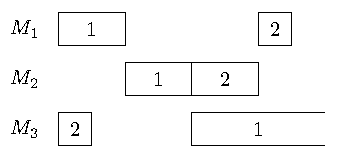
\includegraphics[scale=1]{figures/job-shop-delay.pdf}
  \caption{Example of an optimal schedule for Example~\ref{eg:job-shop}, shown
    as a Gantt chart. Each row $M_{i}$ corresponds to machine $i$ and each block
    numbered $j$ on this row represents the operation $(i,j)$. The dashed lines
    indicate unit time steps. Note that machine 2 is kept idle, while operation
    $(2,2)$ could have already been scheduled at time 1. Furthermore, for this
    particular instance, it can be checked that this is the unique optimal
    schedule.}
  \label{fig:job-shop-delay}
\end{figure}

\paragraph{Disjunctive graph.}

A commonly used representation of job shop problems is through their disjunctive
graph, which is a directed graph with vertices $\mathcal{N}$ corresponding to the
operations and two types of arcs.
%
The conjunctive arcs $\mathcal{C}$ are used to encode the predetermined machine
sequence of each job. Each such arc $(i, j) \rightarrow (k, j)$ encodes that job
$j$ should first be processed on machine $i$ before it is processed on machine
$k$.
%
When two distinct jobs $j_{1}$ and $j_{2}$ both require processing on the same
machine $i$, we say that they are conflicting.
%
The disjunctive arcs $\mathcal{D}$ are used to encode the possible choices of
resolving such conflicts, by deciding which of $j_{1}$ or $j_{2}$ visits $i$
first.
%
More specifically, let $j_{1}$ and $j_{2}$ be conflicting on some machine $i$,
then the nodes $(i,j_{1})$ and $(i,j_{2})$ are connected by two arcs in opposite
directions.

The disjunctive graph can also be used to encode (partial) solutions as follows.
%
It can be shown that each feasible solution corresponds to a selection
$\mathcal{O}$ of exactly one disjunctive arc from each pair such that the
induced graph $(\mathcal{N}, \mathcal{C} \cup \mathcal{O})$ is
acyclic~\cite{pinedoSchedulingTheoryAlgorithms2016}.
%
More precisely, consider two conflicting operations $(i,j_{1})$ and $(i,j_{2})$,
then $\mathcal{O}$ contains either $(i,j_{1}) \rightarrow (i,j_{2})$ or
$(i,j_{1}) \rightarrow (i,j_{2})$.
%
To illustrate this, the empty and complete disjunctive graphs for the instance
in Example~\ref{eg:job-shop} are shown in Figure~\ref{fig:disjunctive-graphs}.

\begin{figure}
  \centering
  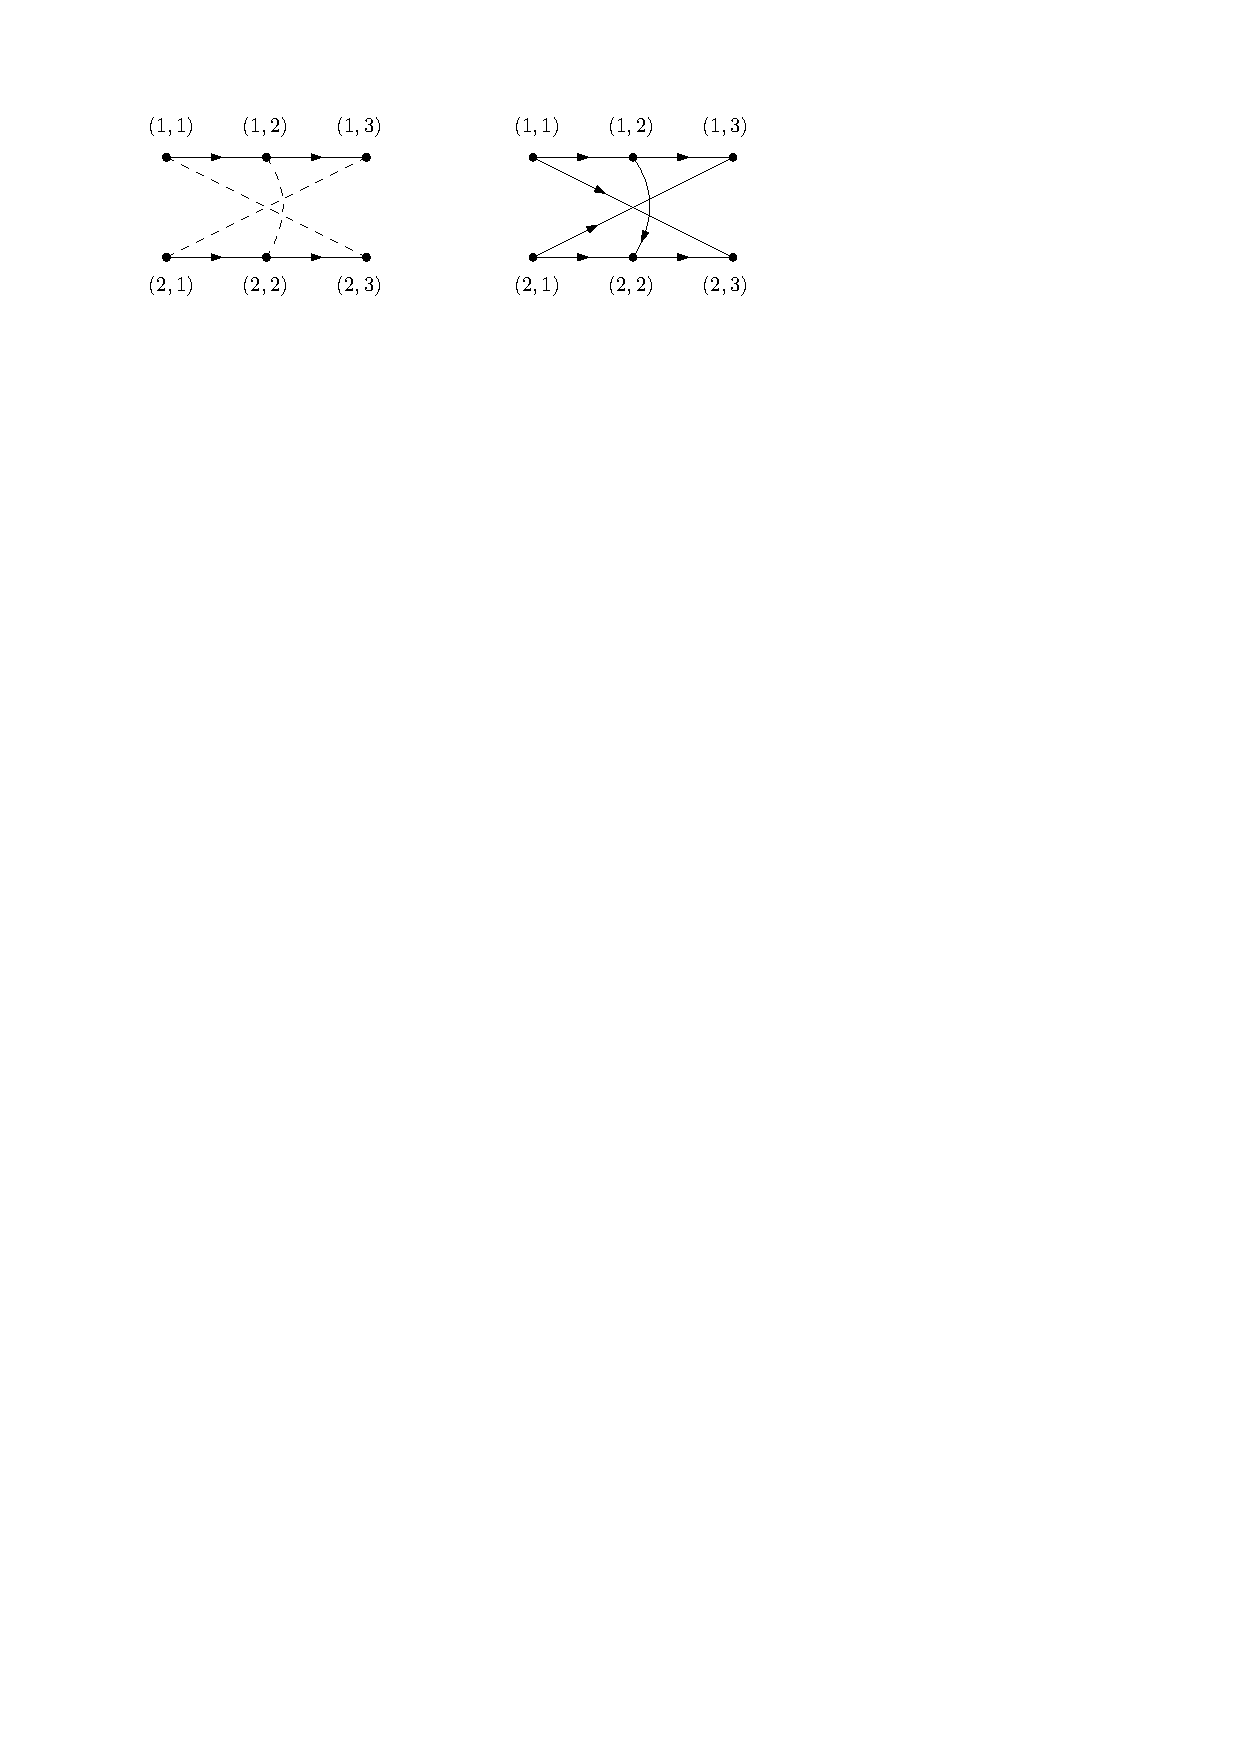
\includegraphics[scale=1]{figures/disjunctive_graph.pdf}
  \caption{Illustration of disjunctive graphs for Example~\ref{eg:job-shop}.
    Horizontal arrows represent conjunctive arcs. We used dashed lines to for
    the pairs of disjunctive arcs as dashed lines. The left graph corresponds to
    an empty selection $\mathcal{O} = \varnothing$ while the right graph shows
    the selection $\mathcal{O}$ that corresponds to the optimal schedule of
    Figure~\ref{fig:job-shop-delay}.}
  \label{fig:disjunctive-graphs}
\end{figure}


\paragraph{Solution methods.}

Most job shop problems are very hard to solve. For example, the class of
problems $Jm|r_{j}|C_{\max}$ considered in Example~\ref{eg:job-shop} is known to
be NP-hard~\cite{grahamOptimizationApproximationDeterministic1979}, even without
release dates, which is denoted $Jm||C_{\max}$.
%
As a consequence, much effort has gone into developing good heurstics.
%
A type of heuristic that is often considered is to apply a so-called \emph{dispatching
rule} in order to build a schedule in a step-by-step fashion.
%
At each step, the rule chooses some job from all jobs with remaining unscheduled
operations and schedules this next operation at the earliest time possible,
given the current schedule.

A more principled way of solving job shop problems relies on the mathematical
programming framework.
%
We illustrate this for the problem $Jm|r_{j}|C_{\max}$ of
Example~\ref{eg:job-shop}. Using the notation of the disjunctive graph, the
problem can be concisely stated as
\[
\renewcommand{\arraystretch}{1.2}
\begin{NiceArray}{ r l @{} >{{}}c<{{}} @{} l @{} }
  \displaystyle \min_{y} & J(y) \\
  \text{such that } \; & y(s_{j},j) \leq r(j) && \quad \text{ for each job } j , \\
  &y(i, j) + p(i, j) \leq y(r, k) && \quad \text{ for each conjunction } (i,j) \rightarrow (r,k) \in \mathcal{C} , \\
  & y(i,j) + p(i,j) \leq y(i,k) & \\
  & \hspace{2em} \text{ or (not both) } && \quad \text{ for each disjunction } (i,j) \leftrightarrow (i,k) \in \mathcal{D} , \\
  & y(i,k) + p(i,k) \leq y(i,j) \\
  & y(i,j) \in \mathbb{R} && \quad \text{ for each operation } (i,j) .
\CodeAfter\SubMatrix.{4-1}{6-2}\}
\end{NiceArray}
\]
%
Note that this is almost an mixed-integer linear program (MILP).
%
Let $M > 0$ be some sufficiently large number and introduce a binary decision
variable $b_{(i,j)\leftrightarrow (i,k)} \in \{0,1\}$ for each pair of
disjunctive arcs, then the pair of disjunctive constraint can be rewritten to
\begin{align*}
  y(i,j) + p(i,j) &\leq y(i,k) + M b_{(i,j)\leftrightarrow (i,k)} , \\
  y(i,k) + p(i,k) &\leq y(i,j) + M (1 - b_{(i,j)\leftrightarrow (i,k)}) ,
\end{align*}
which is generally refered to as the \emph{big-M method}. The resulting MILP can
be solved by any off-the-shelf solver, e.g., we used the commerical Gurobi
Optimizer software~\cite{gurobi} for this thesis.

\section{Reinforcement learning}

For machine learning problems where data-collection is restricted in some way,
the supervised learning paradigm, i.e., learning from labeled examples, is
sometimes no longer appropriate or feasible.
%
Very generally, the reinforcement learning paradigm can viewed as a
generalization of supervised learning in which the data collection and selection
process is not fixed anymore.
%
The classical perspective is that of an \emph{agent} that tries to maximize some
cumulative \emph{rewward} signal when interacting in some \emph{environment},
which is formalized by the Markov Decision Process (MDP) model.
%
We refer the reader to~\cite{suttonReinforcementLearningIntroduction2018} for a
friendly textbook introduction to RL from this perspective.

\paragraph{Problem definition.}
Consider finite sets of states $\mathcal{S}$ and actions $\mathcal{A}$.
%
Given some current state $s$, the agent sends some action $a$ to the
environment, upon which it responds by providing some scalar reward signal $r$
and transitions to state $s'$, which happens with probablity $p(s', r | s, a)$.
%
By fixing a policy $\pi$, which is a function $\pi(a|s)$ that gives the
probablity of the agent choosing action $a$ in state $s$, we obtain the induced
\emph{state Markov chain} with transition probabilities
%
\begin{align*}
  \mathrm{Pr}(s \rightarrow s') = \sum_{a} \sum_{r} \pi(a|s) p(s', r | s, a) .
\end{align*}
Given some initial state distribution $h(s)$, we sample $S_{0} \sim h(s)$ and
use $S_{0}, S_{1}, S_{2}, \dots$ to denote some sample trajectory.
%
Moreover, we can also consider a more fine-grained Markov chain by considering
the sequence of states, actions and rewards
\begin{align*}
  S_{0}, A_{1}, R_{1}, S_{1}, A_{2}, R_{2}, S_{2}, \dots ,
\end{align*}
in which which the state Markov chain is naturally embedded. Such a sample
trajectory is also refered to as an \emph{episode}.
%
Let the corresponding \emph{return} at step $t$ be
defined as
\begin{align*}
  G_{t} = \sum_{k=t+1}^{\infty} R_{k} .
\end{align*}
By marking a subset of states as being \emph{final states}, we can consider finite episodes
\begin{align*}
  S_{0}, A_{1}, R_{1}, S_{1}, A_{2}, R_{2}, S_{2}, \dots S_{N},
\end{align*}
by using the convention that final states return zero reward and transition to
themselves almost surely.
%
For finite episodes, the goal is to find a policy $\pi$ that maximizes the
expected return $\mathbb{E}[G_{0}]$.

\paragraph{Solution methods.}
Most classical methods to find such an optimal policy $\pi$ can be categorized
as either being value-based or policy-based.
%
Value-based can be generally understood as producing some estimate $v(s)$ for
the expected return $\mathbb{E}[G_{0} | S_{0} = s]$. The optimal policy is then
parameterized in terms of these estimates $v(s)$.
%
In contrast, policy-based methods use a more direct parameterization of the
policy space and often rely on some kind of gradient-based optimization.
Specifically, let $\pi_{\theta}$ be some policy with parameters $\theta$, then we aim to
apply the gradient descent updating
\begin{align*}
  \theta \leftarrow \theta - \alpha \nabla \mathbb{E} [ G_{0} ]
\end{align*}
where $\alpha$ is refered to as the learning rate.
%
However, in almost all interesting situations, it is infeasible to compute the
gradient directly.

\section{Neural combinatorial optimization}

% maybe discuss traditional epsilon-approximation schemes?
% argue that it takes a lot of expert knowledge about the problem structure to design these

This section introduces the idea of applying a Machine Learning (ML) perspective
on Combinatorial Optimization (CO) problems, which has gained a lot of
attention recently. One of the key ideas in this line of research is to treat problem
instances as data points and to use machine learning methods to approximately
map them to corresponding optimal solutions~\cite{bengioMachineLearningCombinatorial2020}.

% learning assumptions:
% supervised learning (expert labels) vs reinforcement learning (experience)
\paragraph{Algorithm execution as MDPs.}
It is very natural to see the sequential decision-making process of any
optimization algorithm in terms of the MDP framework, where the environment
corresponds to the internal state of the algorithm. From this perspective, two
main learning regimes can be distinguished.
% imitiation learning
Methods like those based on the branch-and-bound framework are
often computationally too expensive for practical purposes, so \textit{learning
  to imitate} the decisions taken in these exact algorithms might provide us
with fast approximations. In this approach, the ML model's performance is
measured in terms of how similar the produced decisions are to the
demonstrations provided by the expert.
% reinforcement learning
On the other hand, some problems do not even allow efficient exact methods, so it is
interesting to study solution methods that \textit{learn from experience}. An
interesting feature of this direction is that it enables the algorithm to implicitly
learn to exploit the hidden structure of the problems we want to solve.

% neural combinatorial optimization
Because neural networks are commonly used as encoder in these ML models for CO,
we will refer to this new field as \textit{Neural Combinatorial Optimization} (NCO).
%
A wide range of classical combinatorial optimization problems has already been
considered in this framework, so we briefly discuss the taxonomy used in the
survey~\cite{mazyavkinaReinforcementLearningCombinatorial2020}.
% principal vs. joint approach
One distinguishing feature is whether existing off-the-shelf solvers are used or
not. On the one hand, \textit{principal} methods are based on a parameterized algorithm
that is tuned to directly map instances to solutions, while \textit{joint} methods
integrate with existing off-the-shelf solvers in some way (see the
survey~\cite{lodiLearningBranchingSurvey2017} on integration with the
branch-and-bound framework). An illustrative example of the latter category are
the use of ML models for the branching heuristic or the selection of cutting
planes in branch-and-cut algorithms~\cite{tangReinforcementLearningInteger2020}.
% principal - construction vs. improvement (guided search)
The class of principal methods can be further divided into \textit{construction}
heuristics, which produce complete solutions by repeatedly extending partial
solutions, and \textit{improvement} heuristics, which aim at iteratively improving the
current solution with some tunable search procedure.


% learning algorithms:
% REINFOCE with baseline
% Fitting the neural mapping is often done using policy gradient methods (with
% baseline), e.g., with the classical REINFORCE algorithm.

% constraints in differentiable models

\paragraph{Constraint satisfaction.}
A major challenge in NCO is constraint
satisfaction. For example, solutions produced by neural construction policies
need to satisfy the constraints of the original combinatorial problem.
To this
end, neural network components have been designed whose outputs satisfy some
specific type of constraint, for example being a permutation of the
input~\cite{vinyalsPointerNetworks2017a}. Constraints can also be enforced by
the factorization of the mapping into repeated application of some policy. For
example, in methods for TSP, a policy is defined that repeatedly selects the
next node to visit. The constraint that nodes may only be visited once can be
easily enforced by ignoring the visited nodes and taking the argmax among the
model's probabilities for unvisited nodes.

% encoders:
% standard multilayer perceptron networks are not suited to encode order
% pointer networks
% graph neural networks

% backpropagation through solution
Instead of enforcing constraints by developing some tailored model architecture,
like construction and improvement heuristics, general methodologies have
recently been explored for the problem of constraint satisfaction in neural
networks. For example, the DC3 framework~\cite{dontiDC3LearningMethod2021}
employs two differentiable processes, completion and correction, to solve any
violations of equality or inequality constraints, respectively. The more recent
HardNet framework~\cite{minHardConstrainedNeuralNetworks2024} uses a closed-form
projection to map to feasible solutions under affine constraints and relies on a
differentiable convex optimization solver (e.g.,
OptNet~\cite{amosOptNetDifferentiableOptimization2021}) when general convex
constraints are considered.

\subsection{Neural job shop scheduling}

% examples for job-shop scheduling
Various NCO methods have already been studied for JSSP with makespan objective,
of which we now highlight some works that illustrate some of the above classes
of methods. A lot of the policies used in these works rely on some graph neural
network architecture, which is why the survey~\cite{smitGraphNeuralNetworks2024}
provides an overview based on this distinguishing feature.

% Tassel (principal construction, naive environment)
\paragraph{Dispatching rules.}
A very natural approach to model JSSP in terms of an MDP is taken
in~\cite{tasselReinforcementLearningEnvironment2021}, where a dispatching
heuristic is defined in an environment based on discrete scheduling time steps.
%
Every available job corresponds to a valid action and there is a so-called No-Op
action to skip to the next time step. States are encoded by some manually
designed features. They consider the makespan objective by proposing a dense
reward based on how much idle time is introduced compared to the processing time
of the job that is dispatched.
%
In some situation, some action can be proved to be always optimal (``non-final
prioritization''), in which case the policy is forced to take this action.
Additionally, the authors design some rules for when the No-Op action is not
allowed in order to prevent unnecessary idling of machines.
%
The proposed method is evaluated on the widely used
Taillard~\cite{taillardBenchmarksBasicScheduling1993} and
Demirkol~\cite{DEMIRKOL1998137} benchmarks, for which performance is compared to
static dispatching rules and a constraint programming (CP) solver, which is
considered cutting-edge.

% exact start times follow from order
From a scheduling theory
perspective~\cite{pinedoSchedulingTheoryAlgorithms2016}, it can be shown that
optimal schedules are completely characterized by the order of operations for
regular objectives (non-decreasing functions of the completion times). The start
times are computed from this order by a so-called \textit{placement rule}, so
considering discrete time steps introduces unnecessary model redundancy.

% Zhang construction heuristic (principal construction, based on order)

The seminal ``Learning to Dispatch'' (L2D)
paper~\cite{zhangLearningDispatchJob2020} proposes a construction heuristic for
JSSP with makespan objective. Their method is based on a dispatching policy that
is parameterized in terms of a graph neural network encoding of the disjunctive
graph belonging to a partial solution. Again, each action corresponds to
choosing for which job the next operation is dispatched. The rewards are based
on how much the lower bound on the makespan changes between consecutive states.
They use a Graph Isomorphism Network (GIN) architecture to parameterize both an
actor and critic, which are trained using the Proximal Policy Optimization (PPO)
algorithm. Using the Taillard and Demirkol benchmarks, they show that their
model is able to generalize well to larger instances.
% problem with dispatching mechanism
As we already alluded to above, this way of modeling the environment is better
suited to JSSP with regular objectives, because it does not explicitly determine
starting times.
%
They use a dispatching mechanism based on finding the earliest starting time of
a job, even before already scheduled jobs, see their Figure 2. By doing this,
they introduce symmetry in the environment: after operations
$O_{11}, O_{21}, O_{31}$ have been scheduled, both action sequences
$O_{22}, O_{32}$ and $O_{32}, O_{22}$ lead to exactly the same state $S_5$ shown
in their Figure 2. In this particular example, this means that it is impossible
to have $O_{11} \rightarrow O_{22} \rightarrow O_{32}$. In general, it is not
clear whether the resulting restricted policy is still sufficiently powerful, in
the sense that an optimal operation order can always be constructed.

% Zhang improvement heuristic (principal improvement)

\paragraph{Guided local search.}
Recently, the authors of L2D investigated an improvement heuristic for
JSSP~\cite{zhangDeepReinforcementLearning2024} with makespan objective.
%
This method is based on selecting a solution within the well-known $N_5$
neighborhood, which has been used in previous local search heuristics.
%
It is still not clear whether their resulting policy is complete, in the sense
that any operation order can be achieved by a sequence of neighborhood moves.
%
The reward is defined in terms of how much the solution improves relative to the
best solution seen so far (the ``incumbent'' solution). The policy is
parameterized using a GIN architecture designed to capture the topological
ordering of operations encoded in the disjunctive graph of solutions. They
propose a custom $n$-step variant of the REINFORCE algorithm in order to deal
with the sparse reward signal and long trajectories.
%
To compute the starting times based on the operation order, they propose a
dynamic programming algorithm, in terms of a message-passing scheme, as a more
efficient alternative to the classical recursive critical path method.
%
Our proposal for efficiently updating the current starting time lower bounds in
partial solutions can also be understood as a similar message-passing scheme,
but where only some messages are necessary.

\paragraph{Joint method.}
% Tassel (joint with CP solver)
An example of a joint method is given
in~\cite{tasselEndEndReinforcementLearning2023}, where the environment is stated
in terms of a Constraint Programming (CP) formulation. This allows the method to
be trained using demonstration from an off-the-shelf CP solver.


\chapter{Isolated intersection scheduling}\label{chap:single}

\chapter{Learning for the isolated intersection}\label{chap:single-learning}

\section{Reinforcement learning}


For some fixed policy $\pi$ and initial state distribution $h$, we consider the
underlying \textit{induced Markov chain} over states. Because we are working with finite
episodes, the induced state process is a Markov chain with absorbing states.
%
We want to analyze how often states are visited on average, over multiple episodes.
%
To better understand what \textit{on average} means here, imagine that we link
together separate episodes to create a regular Markov chain without absorbing
states, in the following way: from each final state, we introduce state
transitions to the initial states according to distribution $h$, see also
Figure~\ref{fig:episodic_MC}. Furthermore, we will write $S_{t}^{(i)}$ to denote
the state at step $t$ of episode $i$.

\begin{figure}[h]
  \centering
  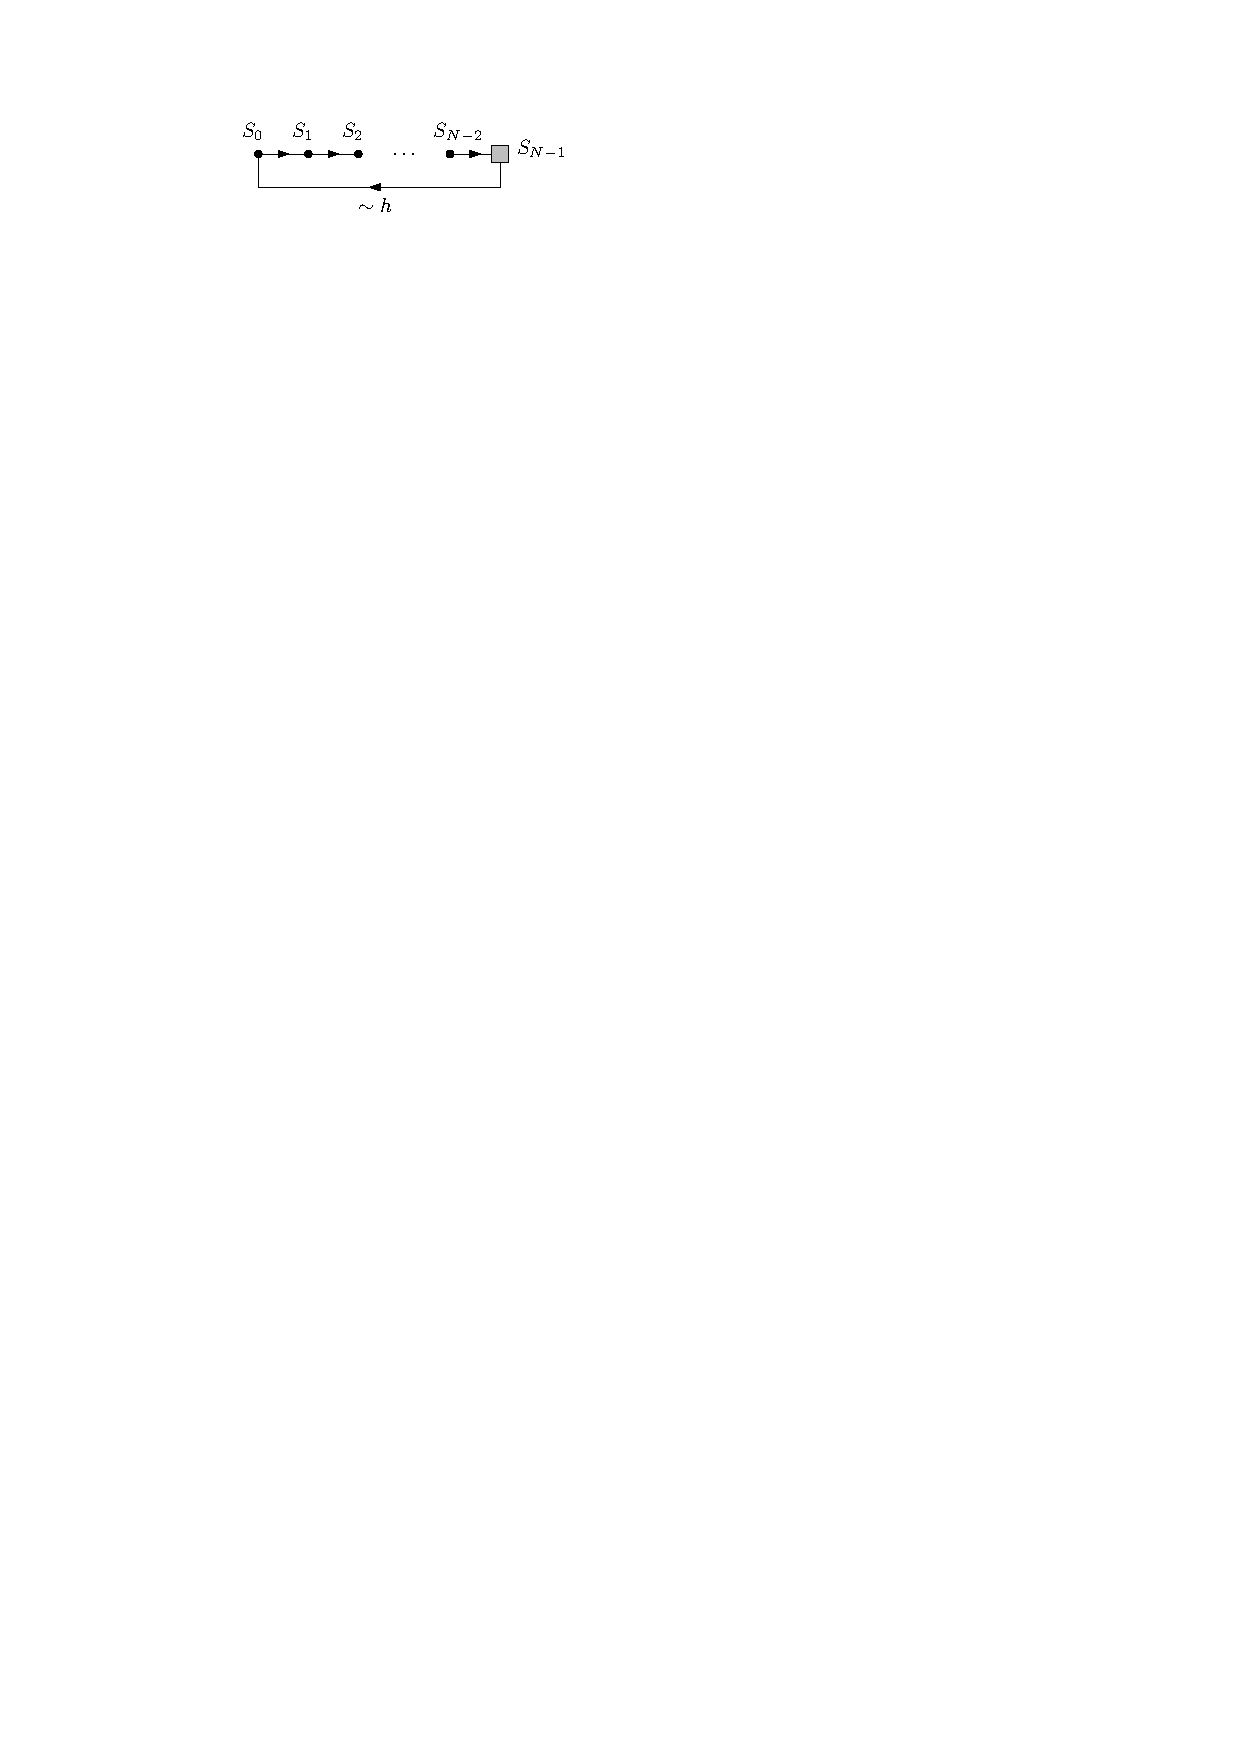
\includegraphics[width=0.4\textwidth]{figures/episodic_markov_chain.pdf}
  \caption{Illustration of the induced Markov chain when dealing with finite
    episodes. The next state after the final state, indicated as the grey
    rectangle, is sampled according to initial state distribution $h$.}
  \label{fig:episodic_MC}
\end{figure}


\paragraph{Stationary distribution for finite episodes.}
Consider an absorbing Markov chain with transition matrix
\begin{align*}
  P_{xy} = \sum_{a} \pi(a | x) p(y | x, a) .
\end{align*}
There are $t$ transient states and $r$ absorbing states, so $P$ can be written
as
\begin{align*}
  P = \begin{pmatrix}
        Q & R \\
        \mathbf{0} & I_{r}
      \end{pmatrix} ,
\end{align*}
where $Q$ is a $t$-by-$t$ matrix, $R$ is a nonzero $t$-by-$r$ matrix, $I_{r}$ is
the $r$-by-$r$ identify matrix and $\mathbf{0}$ is the zero matrix.
%
Observe that $(Q^{k})_{xs}$ is the probability of reaching state $s$ in $k$
steps without being absorbed, starting from state $x$. Hence, the expected
number of visits to state $s$ without being absorbed, starting from state $x$,
is given by
\begin{align*}
  \eta(s | x) := \sum_{k=0}^{\infty} (Q^{k})_{xs} .
\end{align*}
%
Writing this in matrix form $N_{xs} = \eta(s | x)$, we can use the following
property of this so-called Neumann series, to obtain
\begin{align*}
  N = \sum_{k=0}^{\infty} Q^{k} = {(I_{t} - Q)}^{-1} .
\end{align*}
Now we can derive two equivalent equations
\begin{align*}
  N = (I_{t} - Q)^{-1} \iff
  \begin{cases}
    N (I_{t} - Q) = I_{t} \iff N = I_{t} + NQ ,
    \quad  \text{ or }  \\
    (I_{t} - Q) N = I_{t} \iff N = I_{t} + QN . \\
  \end{cases}
\end{align*}
%
Expanding the first equation in terms of matrix entries $N_{xs} = \eta(s | x)$
gives
\begin{align*}
  \eta(s | x) &= \mathds{1}\{ x = s \} + \sum_{y}  \eta(y | x) Q_{ys} \\
  &= \mathds{1}\{ x = s \} +  \sum_{y}\eta(y | x) \sum_{a} \pi(a | y) p(y | x, a)
\end{align*}
and similarly, the second equation gives
\begin{align*}
  \eta(s | x) &= \mathds{1}\{ x = s \} + \sum_{y} Q_{xy} \eta(s | y) \\
  &= \mathds{1}\{ x = s \} +  \sum_{a} \pi(a | x) \sum_{y} p(y | x, a) \eta(s | y)
\end{align*}
%
Now since the initial state is chosen according to distribution $h$, the
expected number of visits $\eta(s)$ to state $s$ in some episode is given by
\begin{align*}
  \eta(s) = \sum_{x} h(x) \eta(s | x) ,
\end{align*}
or written in matrix form $\eta = hN$, where $\eta$ and $h$ are row vectors.
%
Therefore, we can also work with the equations
\begin{align*}
  \begin{cases}
  hN = h + hNQ , \quad \text{ or } \\
  hN = h + hQN ,
  \end{cases}
\end{align*}
which are generally called \textit{balance equations}.
% or written in terms of matrix entries, respectively,
% \begin{align*}
%   \begin{cases}
%   \eta(s) = h(s) + \sum_{x} h(x) \sum_{y} \eta(y|x) \sum_{a} \pi(a|y)p(s|y, a) , \text{ or } \\
%   \eta(s) = h(s) + \sum_{x} h(x) \sum_{a} \pi(a | x) \sum_{y} p(y | x, a) \eta(s | y) .
%   \end{cases}
% \end{align*}
By writing the first variant as $\eta = h + \eta Q$ and expanding the matrix
multiplication, we obtain
\begin{align*}
  \eta(s) = h(s) + \sum_{y} \eta(y) \sum_{a} \pi(a|y)p(s|y,a) .
\end{align*}
%
Through appropriate normalization of the expected number of visits, we obtain
the average fraction of time spent in state $s$, given by
\begin{align*}
  \mu(s) = \frac{\eta(s)}{\sum_{s'} \eta(s')} .
\end{align*}

\paragraph{Monte Carlo sampling.}

Suppose we have some function $f : \mathcal{S} \rightarrow \mathbb{R}$ over
states and we are interested in estimating $\mathbb{E}_{S_{t}^{(i)} \sim \mu}[f(S_{t}^{(i)})]$.
%
We can just take random samples of $S_{t}^{(i)}$, by sampling initial state
$S_{0}^{(i)} \sim h$ and then \textit{rolling out} $\pi$ to obtain
\begin{align*}
\tau^{(i)} = (S_{0}^{(i)},A_{0}^{(i)},R_{1}^{(i)},S_{1}^{(i)},A_{1}^{(i)},R_{2}^{(i)},S_{2}^{(i)}, \dots, S_{N^{(i)}-1}^{(i)}) \sim \pi(\tau^{(i)} | S_{0}^{(i)}),
\end{align*}
where $N^{(i)}$ denotes the total number of states visited in this episode.
%
Given $M$ such episode samples, we compute the estimate as
\begin{align*}
  \mathbb{E}_{S_{t}^{(i)} \sim \mu} [ f(S_{t}^{(i)}) ] \approx \left( \sum_{i=1}^{M} \sum_{t=0}^{N^{(i)} - 1} f(S_{t}^{(i)}) \right) / \left( \sum_{i=1}^{M} N^{(i)} \right) .
\end{align*}

Observe that the analysis of the induced Markov chain can be extended to
explicitly include actions and rewards as part of the state and derive the
stationary distribution of the resulting Markov chain. However, we do not need
this distribution explicitly in practice, because we can again use episode
samples $\tau^{(i)}$. To keep notation concise, we will from now on denote this
type of expectation as $\mathbb{E}_{\tau \sim h,\pi}[f(\tau)]$ and omit episode
superscripts.
%
Using this new notation, note that the average episode length is given by
\begin{align*}
  \mathbb{E}_{h, \pi} [ N ]= \sum_{s'} \eta(s') .
\end{align*}

\subsection{Policy gradient estimation}

Let $v_{\pi_{\theta}} = \mathbb{E}_{h,\pi_{\theta}}[G_{0}]$ denote the expected
episodic reward under policy $\pi$, where $G_{t}$ is called the reward-to-go at
step $t$, which is defined as
\begin{align*}
  G_{t} := \sum_{k=t+1}^{\infty} R_{k} .
\end{align*}
The main idea of policy gradient methods is to update the policy parameters
$\theta$ in the direction that increases the expected episodic reward the most. This
means that the policy parameters are updated as
\begin{align*}
  \theta_{k+1} = \theta_{k} + \alpha \nabla v_{\pi_{\theta}} ,
\end{align*}
where $\alpha$ is the learning rate and the gradient is with respect to
$\theta$. Instead of trying to derive or compute the gradient exactly, we often
use some statistical estimate based on sampled episode. The basic policy
gradient algorithm is to repeat the three steps

\vspace{1em}
\noindent
\hspace*{1em} \texttt{1. sample $M$ episodes $\tau^{(1)}, \dots, \tau^{(M)}$ following $\pi_{\theta}$,}\\
\hspace*{1em} \texttt{2. compute gradient estimate $\widehat{\nabla v_{\pi_{\theta}}}(\tau^{(1)}, \dots, \tau^{(M)})$,} \\
\hspace*{1em} \texttt{3. update $\theta \leftarrow \theta + \alpha \widehat{\nabla v_{\pi_{\theta}}}$.}

\paragraph{REINFORCE estimator.}

We will now present the fundamental policy gradient theorem, which essentially
provides a function $f$ such that
\begin{align*}
  \nabla v_{\pi_{\theta}} = \mathbb{E}_{\tau \sim h,\pi_{\theta}}[f(\tau)] ,
\end{align*}
which allows us to estimate the policy gradient using episode samples.
%
To align with the notation
of~\cite{suttonReinforcementLearningIntroduction2018}, we write
$\mathrm{Pr}(x \rightarrow s, k, \pi) := (Q^{k})_{xs}$, for the probability of
reaching state $s$ in $k$ steps under policy $\pi$, starting from state some
$x$, so that the expected number of visits can also be written as
\begin{align*}
  \eta(s) = \sum_{x} h(x) \sum_{k=0}^{\infty} \mathrm{Pr}(x \rightarrow s, k, \pi)
\end{align*}
%
As proven in the chapter on policy gradient methods
in~\cite{suttonReinforcementLearningIntroduction2018}, the gradient of the value
function for a fixed initial state $s_0$ with respect to the parameters is given
by
\begin{align}
  \nabla v_{\pi}(s_{0}) = \sum_{s} \sum_{k=0}^{\infty} \mathrm{Pr}(s_{0} \rightarrow s, k, \pi) \sum_{a} q_{\pi}(s,a) \nabla \pi(a|s) .
\end{align}
When choosing the initial state $s_{0}$ according to some distribution
$h(s_{0})$, we verify that the final result is still the same as in
\cite{suttonReinforcementLearningIntroduction2018}:
\begin{subequations}
\begin{align}
  \nabla v_{\pi} :=& \nabla \mathbb{E}_{s_{0} \sim h}[v_{\pi}(s_{0})] \\
  =& \sum_{s_{0}} h(s_{0}) \sum_{s} \sum_{k=0}^{\infty} \mathrm{Pr}(s_{0} \rightarrow s, k, \pi) \sum_{a} q_{\pi}(s,a) \nabla \pi(a|s) \\
  =& \sum_{s} \eta(s) \sum_{a} q_{\pi}(s,a) \nabla \pi(a|s) \\
  =& \sum_{s'} \eta(s') \sum_{s} \mu(s) \sum_{a} q_{\pi}(s,a) \nabla \pi(a|s) \\
  \propto& \sum_{s} \mu(s) \sum_{a} q_{\pi}(s,a) \nabla \pi(a|s) ,
\end{align}
\end{subequations}
where the constant of proportionality is just the average episode length.
%
Because we do not know $\mu$ or $q_{\pi}$ explicitly, we would like to estimate
$\nabla v_{\pi}$ based on samples. If we sample episodes according to $h$ and
$\pi$ as explained above, we encounter states according to $\mu$, so we have
\begin{subequations}
\begin{align}
  \nabla v_{\pi} &\propto \mathbb{E}_{h, \pi} \left[ \sum_{a} q_{\pi}(S_{t}, a) \nabla\pi(a | S_{t}) \right] \\
  &= \mathbb{E}_{h, \pi} \left[ \sum_{a} \pi(a | S_{t}) q_{\pi}(S_{t}, a) \frac{\nabla \pi(a | S_{t})}{\pi(a | S_{t})} \right] \\
  &= \mathbb{E}_{h, \pi} \left[ q_{\pi}(S_{t}, A_{t}) \frac{\nabla \pi(A_{t} | S_{t})}{\pi(A_{t}| S_{t})} \right] \\
  &= \mathbb{E}_{h, \pi} \left[ G_{t} \nabla \log \pi(A_{t} | S_{t}) \right] .
  \label{eq:estimator1}
\end{align}
\end{subequations}

\paragraph{Baseline.}
Let $b(s)$ be some function of the state $s$ only, then we have for any $s \in \mathcal{S}$
\begin{align}
  \sum_{a} b(s) \nabla \pi(a | s) = b(s) \nabla \sum_{a} \pi(a | s) = b(s) \nabla 1 = 0 .
\end{align}
This yields the so-called REINFORCE estimate with \textit{baseline}
\begin{subequations}
\begin{align}
  \nabla v_{\pi} &\propto \sum_{s} \mu(s) \sum_{a} (q_{\pi}(s, a) + b(s)) \nabla \pi(a | s) \\
          &= \mathbb{E}_{h, \pi} \left[ \bigl(q_{\pi}(S_{t}, A_{t}) + b(S_{t}) \bigr) \nabla \log \pi(A_{t} | S_{t}) \right] \\
  &= \mathbb{E}_{h, \pi} \left[ \bigl(G_{t} + b(S_{t}) \bigr) \nabla \log \pi(A_{t} | S_{t}) \right] .
  \label{eq:estimator2}
          %&= \mathbb{E}_{h, \pi} \left[ \bigl(G_{t} + b(S_{t}) \bigr) \nabla \log \pi(A_{t} | S_{t}) \right]
\end{align}
\end{subequations}
%
Although estimates~\eqref{eq:estimator1} and~\eqref{eq:estimator2} are both equivalent in terms of their expected
value, they may differ in higher moments, which is why an appropriate choice of
$b$ can make a lot of difference in how well the policy gradient algorithm
converges to an optimal policy.
%
As a specific baseline, consider the expected cumulative sum of rewards up to
step the current step $t$, defined as
\begin{align}
  b(s) = \mathbb{E}_{h,\pi} \left[ \sum_{k=1}^{t} R_{k} \Big| S_{t} = s \right],
\end{align}
then observe that
\begin{subequations}
\begin{align}
  q_{\pi}(s, a) + b(s) &= \mathbb{E}_{h,\pi}\left[ \sum_{k=t+1}^{\infty} R_{k} \Big| S_{t} = s , A_{t} = a \right] + \mathbb{E}_{h,\pi}\left[ \sum_{k=1}^{t} R_{k} \Big| S_{t} = s \right] \\
                     &= \mathbb{E}_{h,\pi}\left[ \sum_{k=1}^{\infty}  R_{k} \Big| S_{t} = s, A_{t} = a \right] \\
                     &= \mathbb{E}_{h,\pi} [ G_{0} | S_{t} = s, A_{t} = a ] ,
\end{align}
\end{subequations}
which is just the expected total episodic reward.
%
Now define function $f$ to be
\begin{subequations}
\begin{align}
  f(s, a) := (q_{\pi}(s, a) + b(s))\nabla \log \pi(a | s) &= \mathbb{E}_{h,\pi} \left[ G_{0} | S_{t} = s, A_{t} = a \right] \nabla \log \pi(a | s) \\
  &= \mathbb{E}_{h,\pi} \left[ G_{0} \nabla \log \pi(a | s) | S_{t} = s, A_{t} = a \right] ,
\end{align}
\end{subequations}
then applying the law of total expectation yields
\begin{align}
  \nabla v_{\pi} \propto \mathbb{E}_{h,\pi}[f(S_{t}, A_{t})] =  \mathbb{E}_{h, \pi} \left[ G_{0} \nabla \log \pi(A_{t} | S_{t}) \right] .
\end{align}


\chapter{Network scheduling}\label{chap:network}


\chapter{Learning for network scheduling}\label{chap:network-learning}

\chapter{Conclusion and discussion}\label{chap:conclusion}

\appendix
\chapter{Feasible configurations for single intersection
  model}\label{app:configuration-space}

\begin{figure}
  \centering
  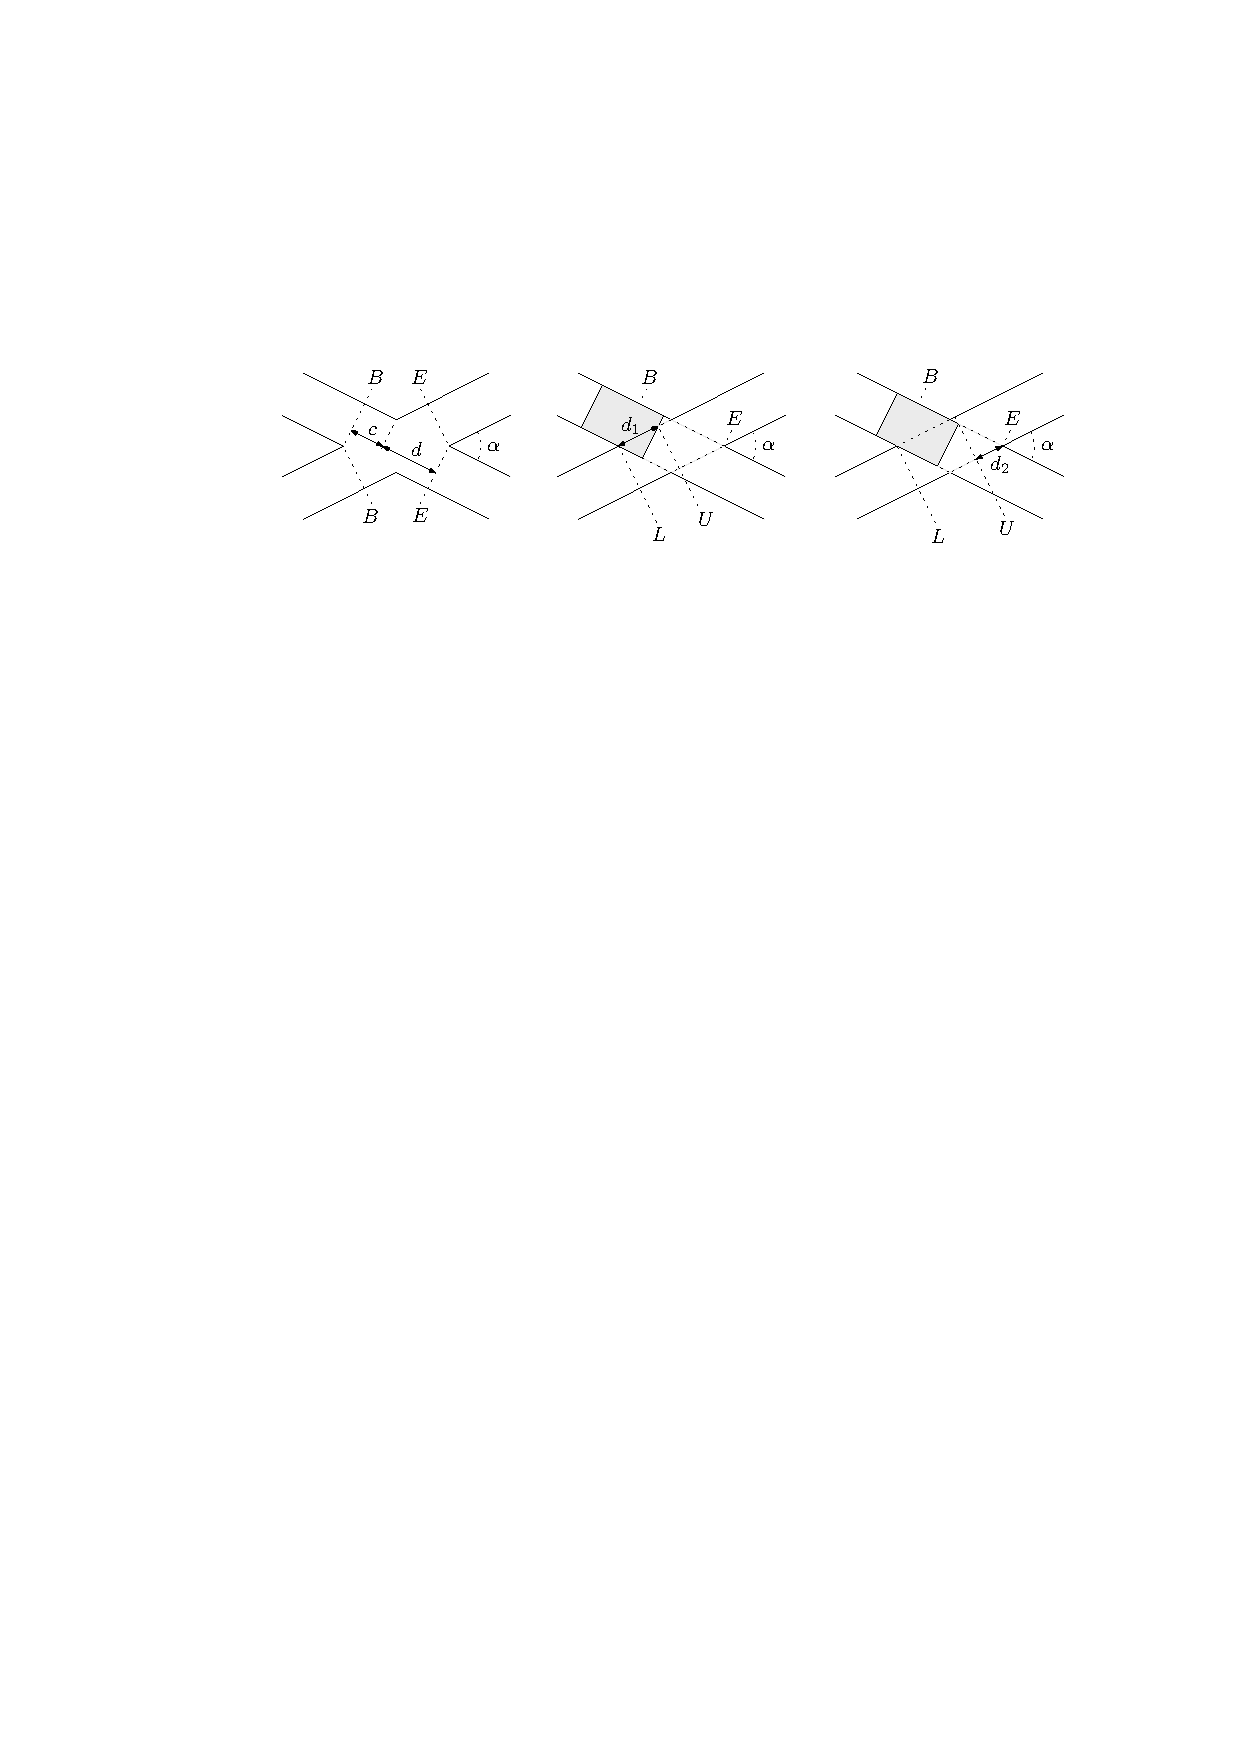
\includegraphics[scale=1]{figures/configuration-space}
  \caption{Sketches to derive the configuration space of the intersection lanes.
    Using some basic trigonometry, the distances in the first figure can be
    shown to be $c = W / \tan(\alpha)$ and $d = W / \sin(\alpha)$. Furthermore,
    observe that we have $(x_{1} - B_{1}) / d_{1} = \cos(\alpha)$ for
    $x_{1} \in \openhalf{B_{1}}{B_{1} + c}$ as shown in the left figures and
    $d_{2}/(E_{1} - x_{1}) = \cos(\alpha)$ for
    $x_{1} \in \halfopen{B_{1} + c}{E_{1}}$ as shown in the right figure. These
    two types of distances can be used to derive the full characterization.}
  \label{fig:configuration-space}
\end{figure}

We provide a possible characterization of the configuration space of the two
lanes that intersect at some arbitrary angle, as shown in
Figure~\ref{fig:intersection-non-axis-aligned}.
% general case
Assume that $\alpha < \pi / 2$ is the acute angle between the two intersections.
We skip a thorough derivation of the following expressions, but we note that it
is based on the type of the distances illustrated in
Figure~\ref{fig:configuration-space}.
%
Roughly speaking, we encode the part of the intersection that vehicle $i=1$
occupies in terms of $x_{2}$ coordinates, by defining the following upper and
lower limit positions
\begin{align}
  U_{1}(x_{1}) &:=
  \begin{cases}
    -\infty & \hspace{1.9em} \text{ if } x_{1} \leq B_{1} \text{ or } x_{1} - L \geq E_{1} , \\
    B_{2} + (x_{1} - B_{1}) / \cos(\alpha) & \hspace{1.9em} \text{ if } x_{1} \in \openhalf{B_{1}}{B_{1} + c\,} , \\
    E_{2} + (x_{1} - E_{1}) \cdot \cos(\alpha) & \hspace{1.9em} \text{ if } x_{1} \in \halfopen{B_{1} + c}{E_{1}} , \\
    E_{2} & \hspace{1.9em} \text{ if } x_{1} \geq E_{1} \text{ and } x_{1} - L < E_{1} ,
  \end{cases} \\
  L_{1}(x_{1}) &:=
  \begin{cases}
    B_{2} & \text{ if } x_{1} - L \leq B_{1} \text{ and } x_{1} > B_{1} , \\
    B_{2} + (x_{1} - L - B_{1}) / \cos(\alpha)     & \text{ if } x_{1} - L \in \openhalf{B_{1}}{E_{1} - c\,} , \\
    E_{2} + (x_{1} - L - E_{1}) \cdot \cos(\alpha) & \text{ if } x_{1} - L \in \halfopen{E_{1} - c}{E_{1}} , \\
    \infty & \text{ if } x_{1} - L \geq E_{1} \text{ or } x_{1} \leq B_{1} .
  \end{cases}
\end{align}
With this definition, $x_{2}$ must satisfy either $x_{2} \leq L_{1}(x_{1})$ or
$x_{2} - L \geq U_{1}(x_{1})$.
%
By symmetry of the system, we define $U_{2}(x_{2})$ and $L_{2}(x_{2})$ by
swapping all indices in the above two expressions and obtain the condition that
$x_{1}$ must satisfy either $x_{1} \leq L_{2}(x_{2})$ or
$x_{1} - L \geq U_{2}(x_{2})$.
%
These two pairs of equations completely characterize the configuration space,
which can now be written as
\begin{align}
  \mathcal{X} = \{ (x_{1}, x_{2}) \in \mathbb{R}^{2} : x_{1} \notin (L_{2}(x_{2}), U_{2}(x_{2})) \text{ and } x_{2} \notin (L_{1}(x_{1}), U_{1}(x_{1})) \}
\end{align}
%
In case the lanes intersect at a right angle $\alpha = \pi / 2$, the situation
is much simpler and the two limiting positions are simply given by
\begin{align}
  (L_{1}, U_{1}) =
  \begin{cases}
    (B_{2},  E_{2})    &\text{ if } (x_{1} - L, x_{1}) \cap (B_{1}, E_{1}) \neq \varnothing , \\
    (\infty, -\infty) &\text{ otherwise, }
  \end{cases}
\end{align}
such that the configuration space is simply given by
\begin{align}
  \mathcal{X} = \mathbb{R}^{2} \setminus ( (B_{1},E_{1}) \times (B_{2}, E_{2}) ) .
\end{align}

\addcontentsline{toc}{chapter}{Bibliography}
\bibliographystyle{unsrt}
\bibliography{references}

\end{document}

% add extra flag when compiling from emacs
% Local Variables:
% TeX-command-extra-options: "-shell-escape"
% End:
